\subsection{附件体检：共同坐标与异常原值}
\label{sec:common-coordinates}

共同首点和超界原值先定义了本节的边界：四谱的共同首点都是 $0\%$ 反射率，附件2另有262个超过 $100\%$ 的原始点，最高约为 $102.74\%$。图~\ref{fig:raw-anomaly}与表~\ref{tab:attachment-check}保留异常的位置与幅值；图中全谱与低波数端放大并列，异常被作为可见的数据事实保留，而不是静默改成缺失。
% src:交接/数据档案.json:总览.零反射率总点数
% src:交接/数据档案.json:总览.超过百分之百总点数;文件档案.1.工作表.0.字段档案.1.统计.最大值;文件档案.1.工作表.0.反射率检查.超过百分之百区段

\begin{figure}[H]
    \centering
    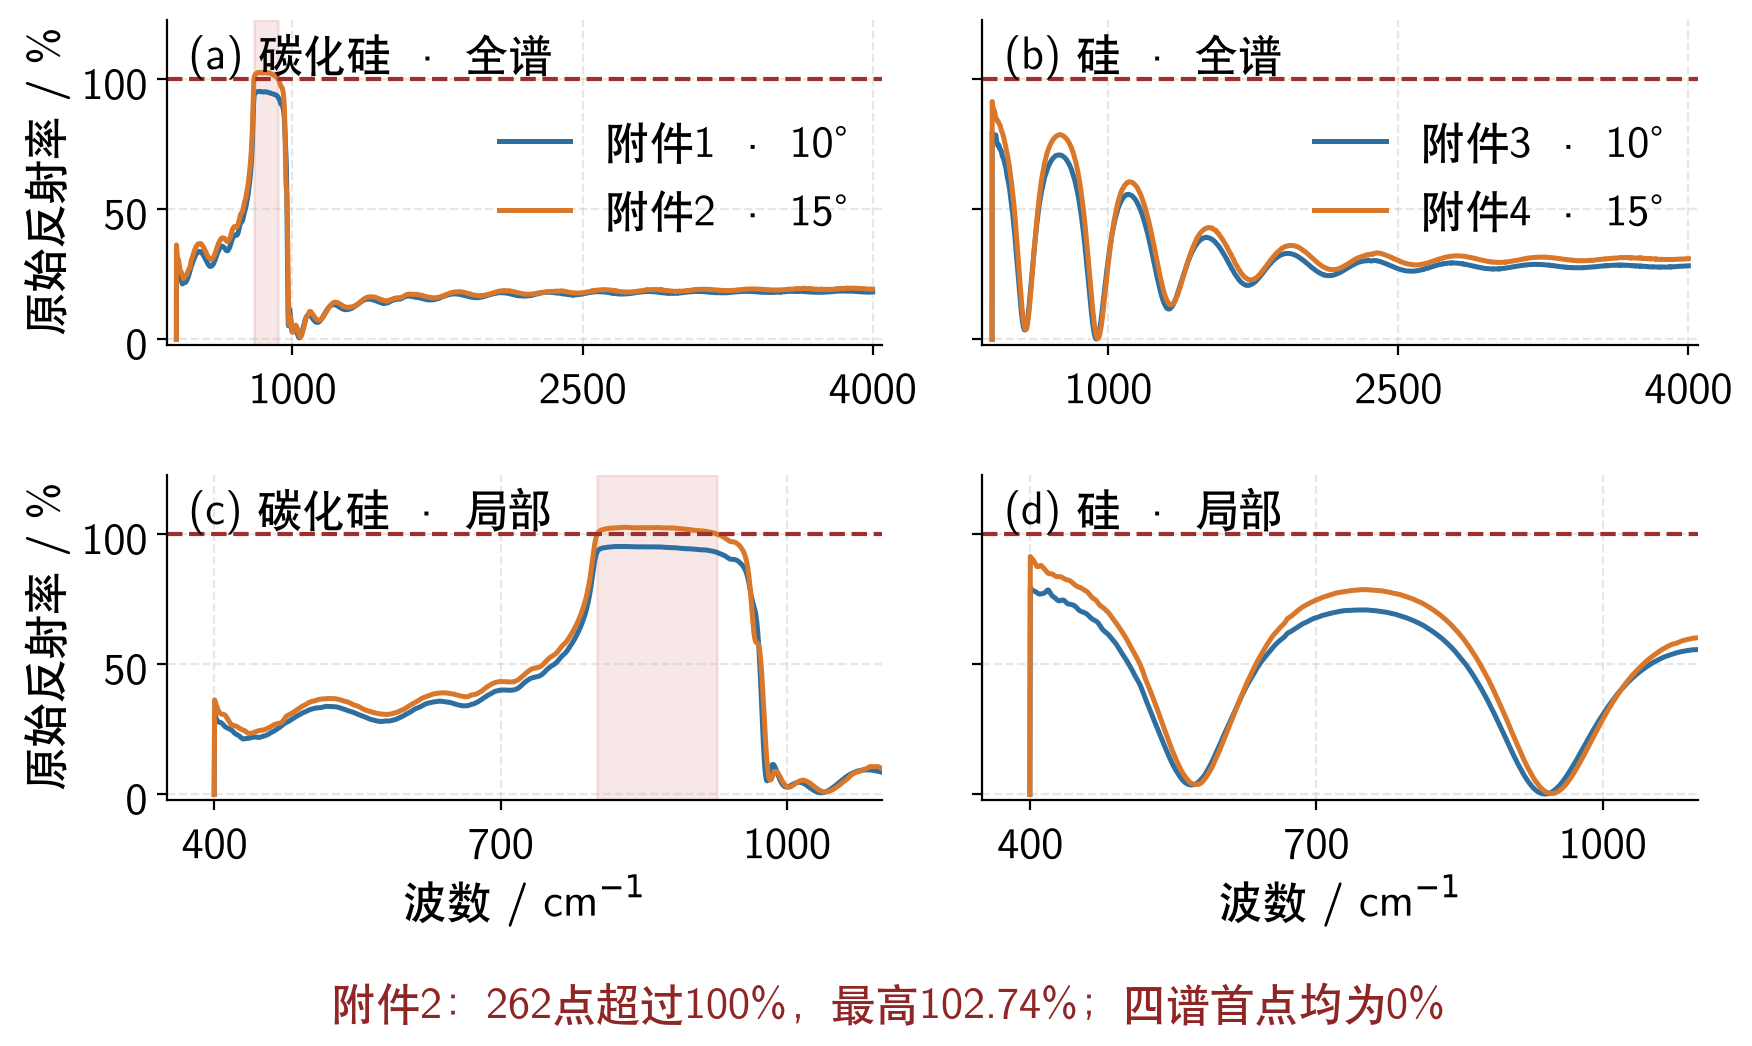
\includegraphics[width=0.96\textwidth]{../求解/公共/图片/四谱原值显示低波数异常.png}
    \caption{四谱原值在低波数端的异常分布}
    \label{fig:raw-anomaly}
\end{figure}

这些质量标记与坐标事实并列后，表~\ref{tab:attachment-check} 给出四谱进入后续比较前的统一口径。

\begin{longtable}{>{\centering\arraybackslash}p{0.20\textwidth}>{\centering\arraybackslash}p{0.24\textwidth}>{\centering\arraybackslash}p{0.24\textwidth}>{\centering\arraybackslash}p{0.20\textwidth}}
\caption{四谱附件体检摘要}\label{tab:attachment-check}\\
\hline
检查对象 & 共同事实 & 质量标记 & 处理口径 \\
\hline
\endfirsthead
\caption[]{四谱附件体检摘要（续）}\\
\hline
检查对象 & 共同事实 & 质量标记 & 处理口径 \\
\hline
\endhead
四谱共同坐标 & 7469点 & 399.67--4000.12~cm$^{-1}$ & 保留原坐标 \\
共同首点 & 4点；$0\%$ & 四谱同首波数 & 标记、保留 \\
附件2超界 & 262点；最高 $102.74\%$ & 801.28--927.11~cm$^{-1}$ & 标记、不裁 \\
主拟合窗口 & 1200--3800~cm$^{-1}$ & 与超界段无交集 & 单独说明 \\
\hline
\end{longtable}
% src:交接/数据档案.json:总览.四文件共有波数点数;总览.波数范围;总览.零反射率总点数
% src:交接/数据档案.json:总览.超过百分之百总点数;文件档案.1.工作表.0.字段档案.1.统计.最大值;文件档案.1.工作表.0.反射率检查.超过百分之百区段
% src:交接/实验记录.json:535.尝试;535.现象;535.决定

四谱各有7469个逐点一致的波数坐标，使双角比较无需插值；相邻步长略有差别，并非严格等间距。曾以端点等距坐标替代原始坐标，发现仍有坐标偏差，因此相位和峰距计算保留原始波数。共同坐标、拟合窗口与质量标记的对照见附录图~\ref{fig:common-coordinate}。
% src:交接/数据档案.json:总览.四文件共有波数点数;总览.波数范围
% src:求解/问题1/结果/实测输入核验.json:共同原始波数点数;波数范围_每厘米
% src:交接/实验记录.json:23.尝试;23.现象;23.决定



主拟合窗口是各模型共同使用的连续波段。低波数端的强烈起伏与中高波数条纹分段处理，高波数末端留作预测核对，主比较沿用原型的 $1200$--$3800\ \mathrm{cm}^{-1}$ 窗口。这两个端点是建模选择，并非裁剪超界点后形成的边界；其对测厚的影响由模型检验章的窗口移动比较考察。
% src:交接/计划.json:统一协议.连续留段.原型与正式区别;问题清单.1.验证方案.防泄漏.2
% src:交接/数据档案.json:文件档案.0.工作表.0.分波段描述
% src:交接/假设台账_问题2.json:5.假设;5.灵敏度义务;5.检验结果

比较按物理范围裁剪与保留原值两种口径后，发现异常段与主拟合窗口不相交，因而保留原始数值并单列质量标记。这里的标记注明异常的位置和幅值，窗外原值仍用于全谱展示与分波段统计。异常区段位于主拟合窗口之外，主拟合使用的原始数值未因此改变。
% src:交接/实验记录.json:535.尝试;535.现象;535.决定
% src:交接/图注素材_1.json:1.独有信息;3.独有信息

问题三的硅全量在同一窗口每角保留5392个原始点。
% src:求解/问题3/结果/解读核验_回炉3_仲裁后.json:防泄漏.全量每角点数

量纲也在此处锁定：反射率按百分数记录，计算按比例使用；波数保持 $\mathrm{cm}^{-1}$，厚度进入传播相位时用 $\mathrm{cm}$，输出再换成 $\mu\mathrm{m}$。因此，原值遵循“只标不裁”，坐标遵循“逐点对齐”；下一节据此检查不同波段的散布是否能够共用一个尺度，并核对光学参数缺口。
% src:交接/假设台账_问题1.json:1.假设
